%%% ======= Beamer ======
\documentclass[usenames,dvipsnames,t]{beamer}
% \documentclass[usenames,dvipsnames, handout]{beamer}
\beamertemplatenavigationsymbolsempty % remove toolbar at the bottom of slides
\usepackage{appendixnumberbeamer} % for appendix
\usetheme{Madrid}
\usecolortheme{default}
\useinnertheme{circles}

\usepackage{fontawesome}

% Define commands for social media icons with links
\newcommand{\twitter}{\href{https://twitter.com/ThibeauWouters}{\textcolor{black}{\faTwitter}}}
\newcommand{\linkedin}{\href{https://www.linkedin.com/in/ThibeauWouters}{\textcolor{black}{\faLinkedin}}}
\newcommand{\github}{\href{https://github.com/ThibeauWouters}{\textcolor{black}{\faGithub}}}
\newcommand{\myemail}{\href{mailto:t.r.i.wouters@uu.nl}{\textcolor{black}{\faEnvelope}}}

\definecolor{customblue}{HTML}{7db8dc}
\newcommand{\thetaeos}{\boldsymbol{\theta}_{\rm{EOS}}}
\newcommand{\boldtheta}{\boldsymbol{\theta}}

\newcommand{\bayesfactor}{\mathcal{B}}

\setbeamercolor{author in head/foot}{bg=blue!10, fg=blue}
\setbeamercolor{title in head/foot}{bg=blue!10, fg=blue}
\setbeamercolor{date in head/foot}{bg=blue!10, fg=blue}

\makeatletter
\setbeamertemplate{footline}{
  \leavevmode%
  \hbox{%
  \begin{beamercolorbox}[wd=.333333\paperwidth,ht=2.25ex,dp=1ex,center]{author in head/foot}%
    \usebeamerfont{author in head/foot}\insertshortauthor\expandafter\ifblank\expandafter{\beamer@shortinstitute}{}{~~(\insertshortinstitute)}
  \end{beamercolorbox}%
  \begin{beamercolorbox}[wd=.333333\paperwidth,ht=2.25ex,dp=1ex,center]{title in head/foot}%
    \usebeamerfont{title in head/foot}\insertshorttitle
  \end{beamercolorbox}%
  \begin{beamercolorbox}[wd=.333333\paperwidth,ht=2.25ex,dp=1ex,right]{date in head/foot}%
    \usebeamerfont{date in head/foot}\insertshortdate{}\hspace*{2em}
    \insertframenumber{}%
%     / \inserttotalframenumber
    \hspace*{2ex} 
  \end{beamercolorbox}}%
  \vskip0pt%
}
\makeatother

% Show the TOC at the beginning
\AtBeginSection[]{
  \addtocounter{framenumber}{-1}
  \begin{frame}
      \frametitle{Contents}
      \tableofcontents[currentsection,subsectionstyle=shaded/shaded/hide]
  \end{frame}
}


\colorlet{beamer@blendedblue}{blue!70} % change color theme

\usepackage[style=numeric-comp,sorting=none,backend=biber]{biblatex}%<- specify style
\addbibresource{references.bib}%<- specify bib file

\usepackage[inkscapearea=page]{svg}
\usepackage{adjustbox}


% For appendix
\newcommand{\backupbegin}{
   \newcounter{framenumberappendix}
   \setcounter{framenumberappendix}{\value{framenumber}}
}
\newcommand{\backupend}{
   \addtocounter{framenumberappendix}{-\value{framenumber}}
   \addtocounter{framenumber}{\value{framenumberappendix}} 
}

\setbeamertemplate{bibliography item}{\insertbiblabel} % improved references



% Other preamble stuff:
\usepackage{preamble}

%%% Uncomment for another color palette
% \definecolor{Logo1}{rgb}{0.0, 0, 0.7}
% \definecolor{Logo2}{rgb}{2.55, 2.55, 2.55}

% \setbeamercolor*{palette primary}{bg=Logo1, fg=white}
% \setbeamercolor*{palette secondary}{bg=Logo2, fg=white}
% \setbeamercolor*{palette tertiary}{bg=white, fg=Logo1}
% \setbeamercolor*{palette quaternary}{bg=white,fg=white}
% \setbeamercolor{structure}{fg=Logo1} % itemize, enumerate, etc
% \setbeamercolor{section in toc}{fg=Logo1} % TOC sections

% For figures
\usepackage{import}
\usepackage{xifthen}
\usepackage{pdfpages}
\usepackage{transparent}
\usepackage{mdframed}
\usepackage{subcaption}

\setbeamertemplate{caption}[numbered]



% --- Inkscape figures:
\newcommand{\incfig}[2][0.75\textwidth]{%
    \def\svgwidth{\columnwidth}
    \resizebox{#1}{!}{\import{Inkscape/}{#2.pdf_tex}}
}

% --- Height of frame
\newlength{\myheight}
\setlength{\myheight}{7cm}

\newlength\myheightfigureintext
\newlength\mydepthfigureintext
\settototalheight\myheightfigureintext{Xygp}
\settodepth\mydepthfigureintext{Xygp}
\setlength\fboxsep{0pt}

\usepackage{tikz}
\usepackage[absolute,overlay]{textpos} % for precise positioning


%------------------------------------------------------------
%This block of code defines the information to appear in the
%Title page
\title[] %optional
{From constraints to classifications: closing the loop in neutron star data analysis}

\author[Thibeau Wouters]{Thibeau Wouters \\ \vspace{2mm} \href{mailto:t.r.i.wouters@uu.nl}{t.r.i.wouters@uu.nl} \newline \github \quad \linkedin \quad \twitter \myemail}


\date{AIslands 2025}

%End of title page configuration block
%------------------------------------------------------------



%------------------------------------------------------------
%The next block of commands puts the table of contents at the 
%beginning of each section and highlights the current section:

%------------------------------------------------------------


\begin{document}

{
\usebackgroundtemplate{\transparent{0.85}{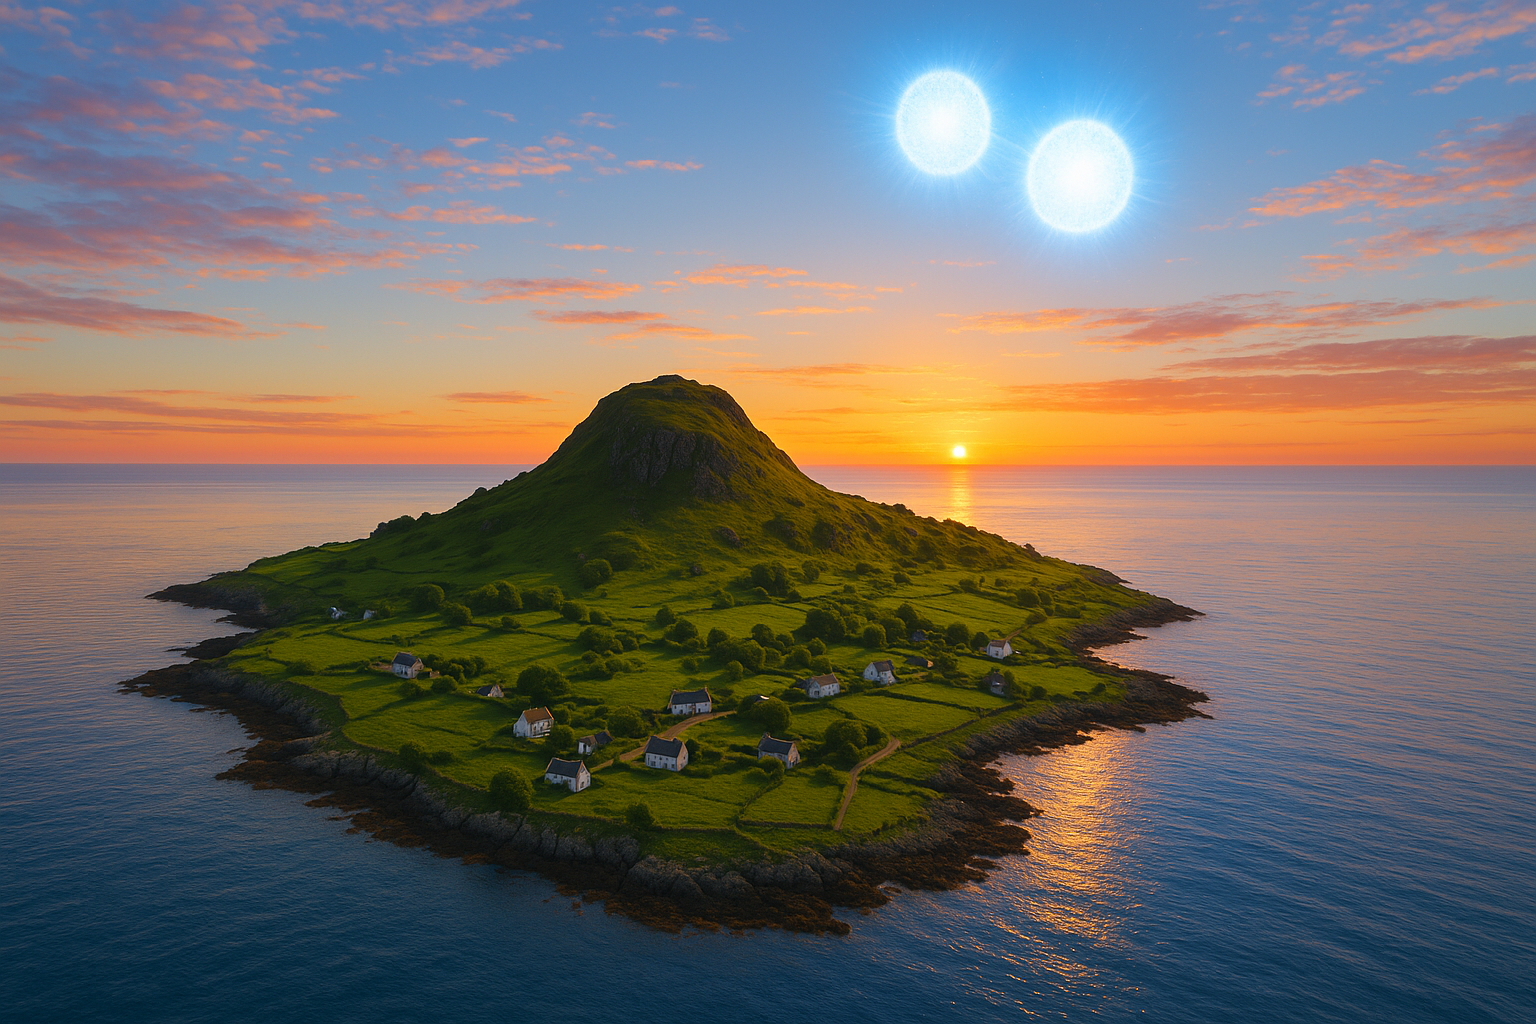
\includegraphics[width=\paperwidth,height=\paperheight]{Figures/AIslands_cover_4.png}}}

% \begin{frame}[plain]
% \titlepage

% \end{frame}
\begin{frame}[plain, noframenumbering]

  \begin{tikzpicture}[remember picture,overlay]
    \node[fill=customblue, fill opacity=0.75, text opacity=1, rounded corners=10pt, inner sep=15pt] at (current page.center) {
      \begin{minipage}{0.8\textwidth}
        \centering
        \textbf{From constraints to classifications: closing the loop in neutron star data analysis}\\[1.5ex]
        \normalsize Thibeau Wouters \\[0.5ex]
        \github \quad \linkedin \quad \twitter \quad \myemail
      \end{minipage}
    };
  \end{tikzpicture}
  
  \vspace{7cm}

  \begin{columns}
  \column{0.35\textwidth}
  \begin{figure}
    \centering
    \vspace{1.5mm}
    
\includegraphics[width=0.75\linewidth]{Figures/utrecht-university.png}
  \end{figure}
  \column{0.35\textwidth}
  \begin{figure}
    \centering
    
\includegraphics[width=0.75\linewidth]{Figures/Nikhef_logo-transparent.png}
  \end{figure}
\end{columns}
  
  \end{frame}
}

% %The next statement creates the title page.
% \frame[plain]{\titlepage
% }


%---------------------------------------------------------
%This block of code is for the table of contents after the title page
% \begin{frame}[plain, noframenumbering]
% \frametitle{Table of Contents}
% \tableofcontents
% \end{frame}
%---------------------------------------------------------


\begin{frame}{The equation of state (EOS)}
  \def\x{2mm}
  \def\y{2mm}

  \begin{itemize}
    \item The equation of state (EOS) of dense nuclear matter is still uncertain~\cite{Koehn:2024set}

    \vspace{\x}

    \item Neutron star (NS) properties depend on the EOS: probe its high density regime ($2$-$8$ $n_{\rm{sat}}$)
  \end{itemize}

  \vspace{\x}

  \begin{figure}
    \centering
    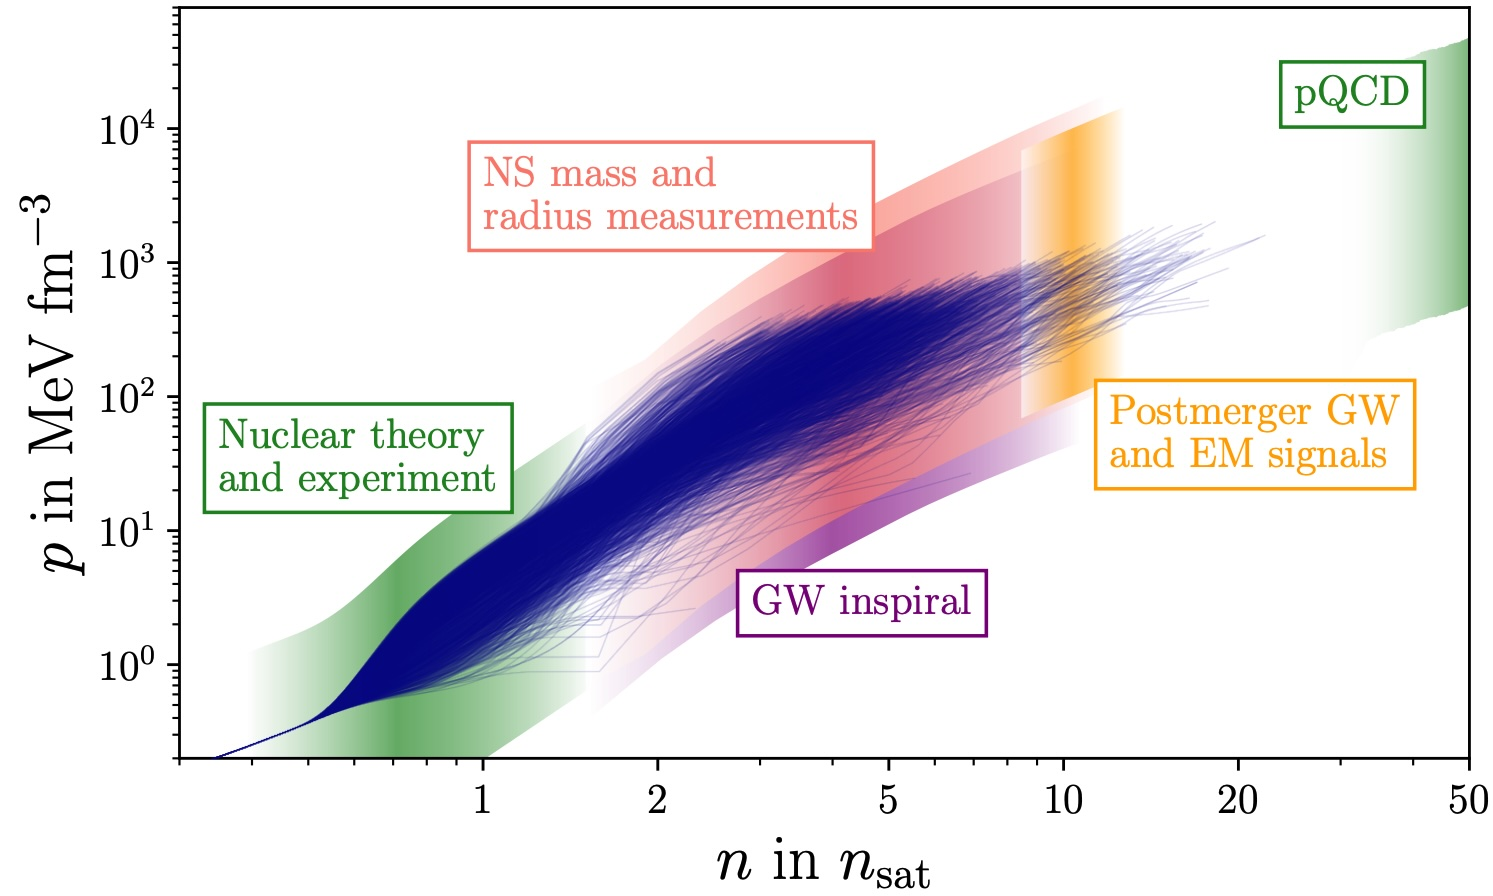
\includegraphics[width=0.75\linewidth]{Figures/Koehn_EOS.jpg} 
  \end{figure}
\end{frame}

\begin{frame}{Structure of this talk}
  \def\x{2mm}
\def\y{1mm}

Data analysis of neutron stars forms a \textbf{loop}:

\vspace{\y}
\begin{enumerate}
    \item \red{Constraining} the EOS with neutron star observations

    \vspace{\x}
    
    \item \red{Applying} EOS knowledge in neutron star data analysis (e.g., GW)
\end{enumerate}

\vspace{\x}

How can we efficiently perform this loop?

\vspace{\y}

\centering
\incfig[0.9\textwidth]{NS_to_EOS}    
\end{frame}

\section{Constraining the EOS}

\begin{frame}{Constraining the EOS}
  \def\x{2mm}
  \def\y{5mm}

  \begin{itemize}
    \item EOS determined with Bayesian inference:
    \begin{align*}
      \mathcal{P}(\theta_{\rm{EOS}} | d ) &\propto \red{\mathcal{L}(d | \theta_{\rm{EOS}})} \pi(\theta_{\rm{EOS}}) \\
      \rm{posterior} &\propto \rm{\red{likelihood}} \times \rm{prior}
    \end{align*}

    \vspace{\x}

    \item The TOV equations predict NS properties as function of EOS

    \vspace{\x}

    \item Solving the TOV equations is slow: \red{costly likelihood} evaluation! Use ML?

    % \vspace{\x}

    % \item How can we accelerate this process?
  \end{itemize}

  \vspace{\y}

  \centering
  \incfig[0.95\textwidth]{NS_likelihood}

\end{frame}

\begin{frame}{\textsc{Jester}: accelerated TOV solvers}
  \def\negx{-3mm}
  \def\x{4mm}
  \def\z{1mm}

  \vspace{\negx}

  \begin{columns}
    \begin{column}{0.80\textwidth}

      \textsc{Jester}~\cite{Wouters:2025zju}: fast EOS code and TOV solver with \textsc{Jax}
      \begin{itemize}
        \item GPU acceleration

        \vspace{\z}

        \item Just-in-time (JIT) compilation

      \end{itemize}
    \end{column}

    \vspace{\x}

    \begin{column}{0.20\textwidth}
      \begin{figure}
        \centering
      
\includegraphics[width=0.75\linewidth]{Figures/jax.png}
      \end{figure}
    \end{column}
  \end{columns}

  \begin{tcolorbox}[colback=blue!10, boxrule=0pt]
    \textsc{Jester} achieves same speed as machine learning surrogates!
  \end{tcolorbox}

  \vspace{\negx}

  \begin{figure}
    \centering
    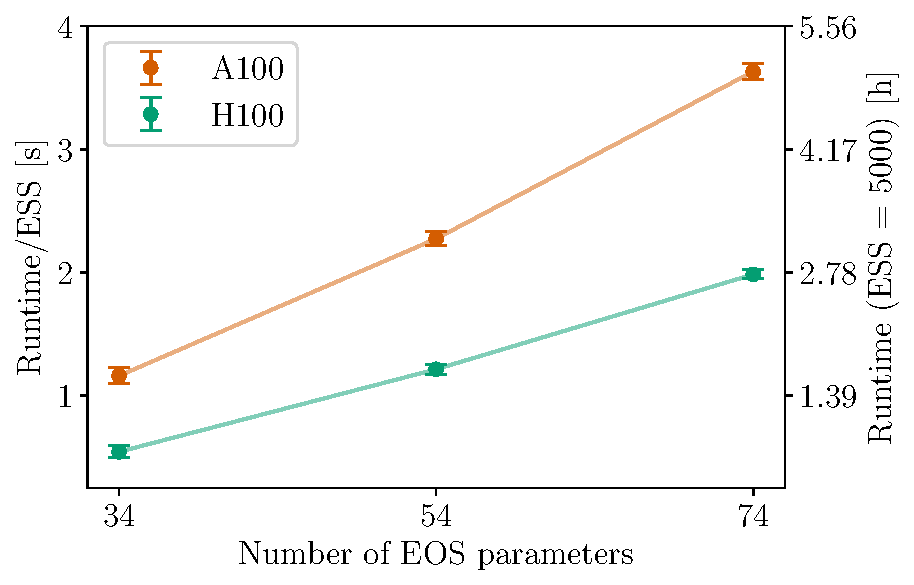
\includegraphics[width=0.60\linewidth]{Figures/scaling_plot.pdf}
  \end{figure}
\end{frame}

% \begin{frame}{Two sets of EOS constraints}
%   \def\x{3mm}
%   \def\y{-4mm}

%   \begin{columns}[T]
%     \column{0.49\textwidth}
%     \vspace{\y}

%     \begin{itemize}
%       \item $M_{\rm{max}} > 2 M_\odot$
%     \end{itemize}

%     \begin{figure}
%       \centering
%       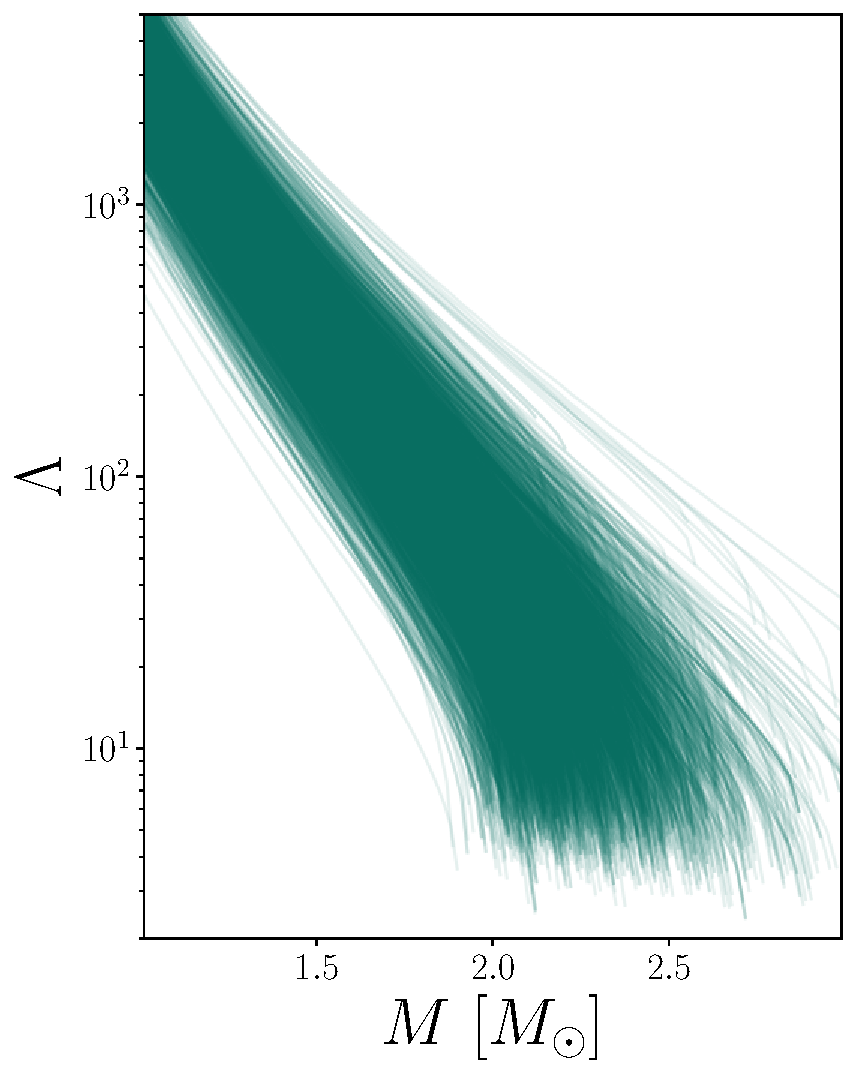
\includegraphics[width=0.85\linewidth]{Figures/lambda_curves.pdf}
%     \end{figure}

%     \column{.01\textwidth}
%     \rule{.2mm}{.8\textheight}

%     \column{0.49\textwidth}
%     \vspace{\y}

%     \begin{itemize}
%       \item $M_{\rm{max}} > 2 M_\odot$
%       \item Nuclear theory predictions
%       \item Mass-radius measurements
%       \item GW170817
%     \end{itemize}
    
%     \vspace{\y}
    
%     \centering 
%     \begin{figure}
%       \centering
%       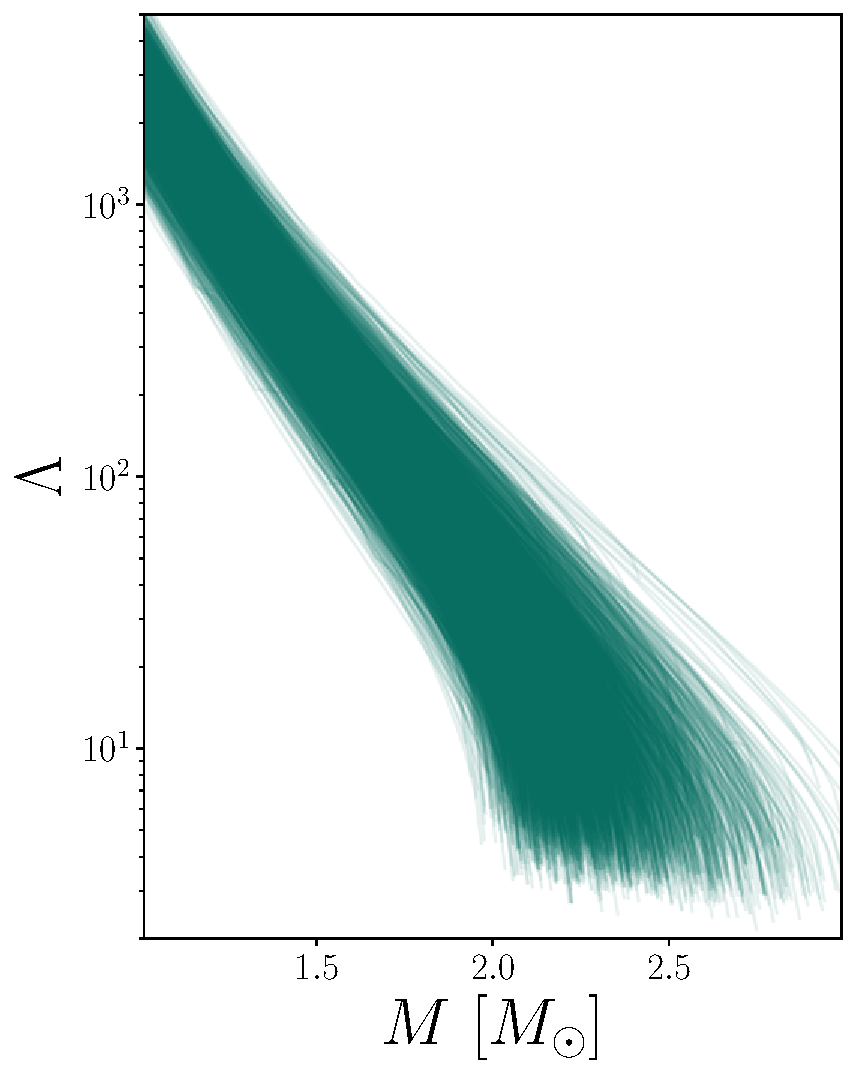
\includegraphics[width=0.85\linewidth]{Figures/lambda_curves_all.pdf}
%     \end{figure}
%   \end{columns}
% \end{frame}


\section{Applying EOS knowledge in GW data analysis}

\begin{frame}[plain, noframenumbering]{Structure of this talk}
  \def\x{2mm}
\def\y{1mm}

Data analysis of neutron stars forms a \textbf{loop}:

\vspace{\y}
\begin{enumerate}
    \item \red{Constraining} the EOS with neutron star observations

    \vspace{\x}
    
    \item \red{Applying} EOS knowledge in neutron star data analysis (e.g., GW)
\end{enumerate}

\vspace{\x}

How can we efficiently perform this loop?

\vspace{\y}

\centering
\incfig[0.9\textwidth]{NS_to_EOS}    
\end{frame}

\begin{frame}{Tidal deformability}
  \def\x{4mm}

  \begin{itemize}
    \item Neutron stars are tidally deformed in a binary
    
    \vspace{\x}
    
    \item Quantified by the tidal deformability $\Lambda$

    \vspace{\x}

    \item Depends on the EOS: $\Lambda = \Lambda(m, \rm{EOS})$ (black holes: $\Lambda = 0$)

    \vspace{\x}

    \item Imprint in the GW phase: $\tilde{\Lambda}(m_i, \Lambda_i)$ %  $\rightarrow$ measurable $\rightarrow$ EOS constraints
  \end{itemize}

  \begin{figure}
    \centering
    \incfig[1.0\textwidth]{tidal}
  \end{figure}
\end{frame}


\begin{frame}{Equation of state-informed priors}
  \def\x{4mm}
  \def\y{1mm}

  \begin{itemize}
    \item GW parameters are determined with Bayesian inference:
    \begin{align*}
      \mathcal{P}(\theta_{\rm{GW}} | d ) &\propto \mathcal{L}(d | \theta_{\rm{GW}}) \red{\pi(\theta_{\rm{GW}})} \\
      \rm{posterior} &\propto \rm{likelihood} \times \rm{\red{prior}} \\
    \end{align*}

    \vspace{-4mm}

    \item By default, we choose \textbf{\jaxthree{agnostic priors}}: e.g. $\Lambda_i \sim \mathcal{U}(0, 5000)$

    \vspace{\x}
    \pause

    \item \textbf{But}, we have prior knowledge from the EOS:
    \begin{itemize}
      \vspace{\y}
      \item Masses $m_i$ determined by $M_{\rm{max}}$

      \vspace{\y}

      \item $\Lambda_i$ determined by $m_i$ and EOS
    \end{itemize}
    
    \vspace{\x}
    
    \item \textbf{\jaxtwo{Equation of state-informed prior}}:
    \begin{align*}
      \pi(m_1, m_2, \Lambda_1, \Lambda_2) = \int \diff \theta_{\rm{EOS}} \ &\pi(m_1, m_2 | \theta_{\rm{EOS}}) \pi(\Lambda_1, \Lambda_2 | m_1, m_2, \theta_{\rm{EOS}}) \\
      &\times \pi(\theta_{\rm{EOS}})
    \end{align*}
  \end{itemize}
\end{frame}

\begin{frame}{Equation of state-informed priors}
  \def\x{2mm}
  \def\y{2mm}

  \begin{itemize}
    \item Example: EOSs with $M_{\rm{max}} > 2.0 M_\odot$
    
    % \vspace{\x}
    
    % \item This gives a prior $\pi(m_1, m_2, \Lambda_1, \Lambda_2)$ for binary neutron star mergers

    \vspace{\x}

    \item Emulate $\pi(m_1, m_2, \Lambda_1, \Lambda_2)$  with a \textbf{\jaxtwo{normalizing flow}}
  \end{itemize}

  \vspace{\y}

  \centering
  \incfig[0.975\textwidth]{NFprior}
\end{frame}

\begin{frame}{Posterior for single injection}
  \def\x{2mm}

  \begin{itemize}
    \item \textbf{\jaxthree{Agnostic}}: uniform prior for chirp mass, mass ratio, $\Lambda_1$, $\Lambda_2$

    \vspace{\x}

    \item \textbf{\jaxtwo{Data-driven}}: normalizing flow prior $\pi(m_1, m_2, \Lambda_1, \Lambda_2)$

    \vspace{\x}

    \item Tidal content of source more constrained (SNR = 13)

    \vspace{\x}
  \end{itemize}

  \begin{figure}
    \centering
    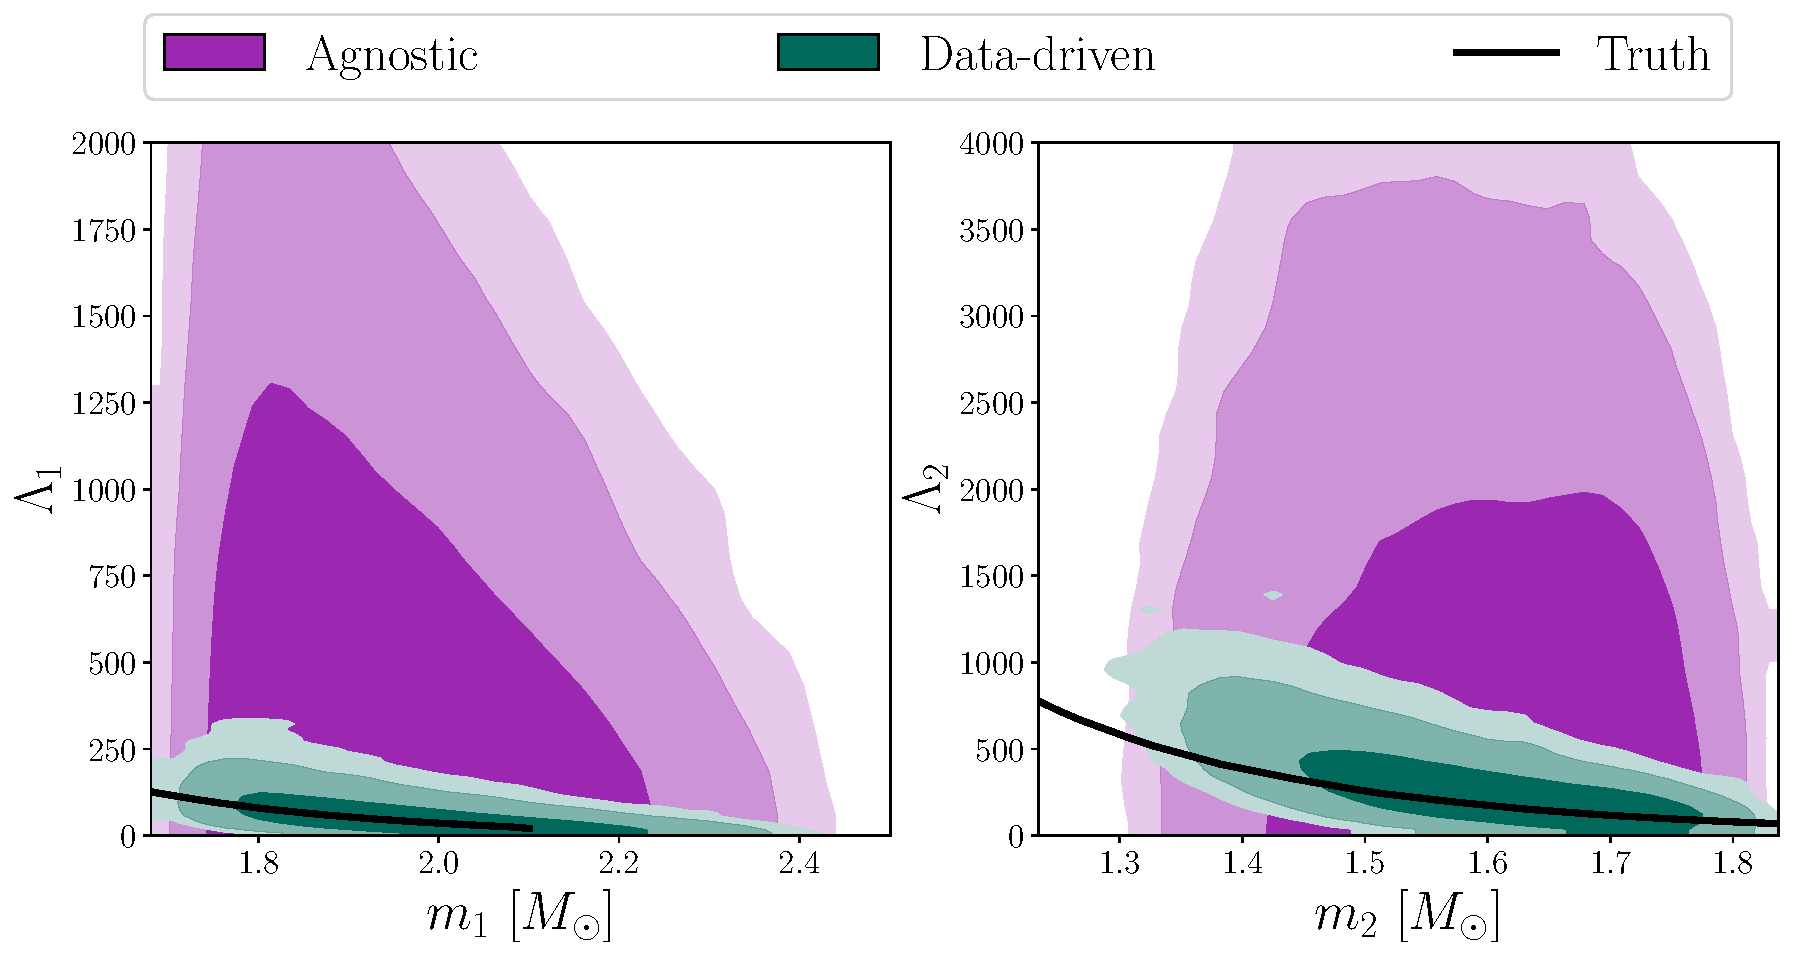
\includegraphics[width=0.875\linewidth]{Figures/jester_Aplus_2.pdf}
  \end{figure}
\end{frame}


\begin{frame}{Source classification}
  \def\x{2mm}

  \begin{itemize}
    \item Similar to the \textbf{\jaxtwo{binary neutron star (BNS)}} prior, we can also construct a \textbf{\nsbh{neutron star-black hole (NSBH)}} prior

    \vspace{\x}
  
    \item Use EOS constraints to classify mergers
  \end{itemize}

  \vspace{\x}

  \centering
  \incfig[0.95\textwidth]{bns_vs_nsbh}
\end{frame}

\begin{frame}{Source classification: proof of concept}
  \def\x{3mm}
  \def\y{-2mm}

  \begin{columns}[T]
    \column{0.49\textwidth}
    \centering 
    \textbf{GW170817}
    \vspace{\x}
    \begin{align*}
      ln \ \bayesfactor^{\jaxtwo{\rm{BNS}}}_{\nsbh{\rm{NSBH}}} &= 44.75 \\
      ln \ \bayesfactor^{\jaxtwo{\rm{BNS}}}_{\jaxthree{\rm{agnostic}}} &= 2.83
      % ln \ \bayesfactor^{\nsbh{\rm{NSBH}}}_{\jaxthree{\rm{agnostic}}} &= -41.92 \\
    \end{align*}

    \vspace{\y}

    \begin{figure}
      \centering
      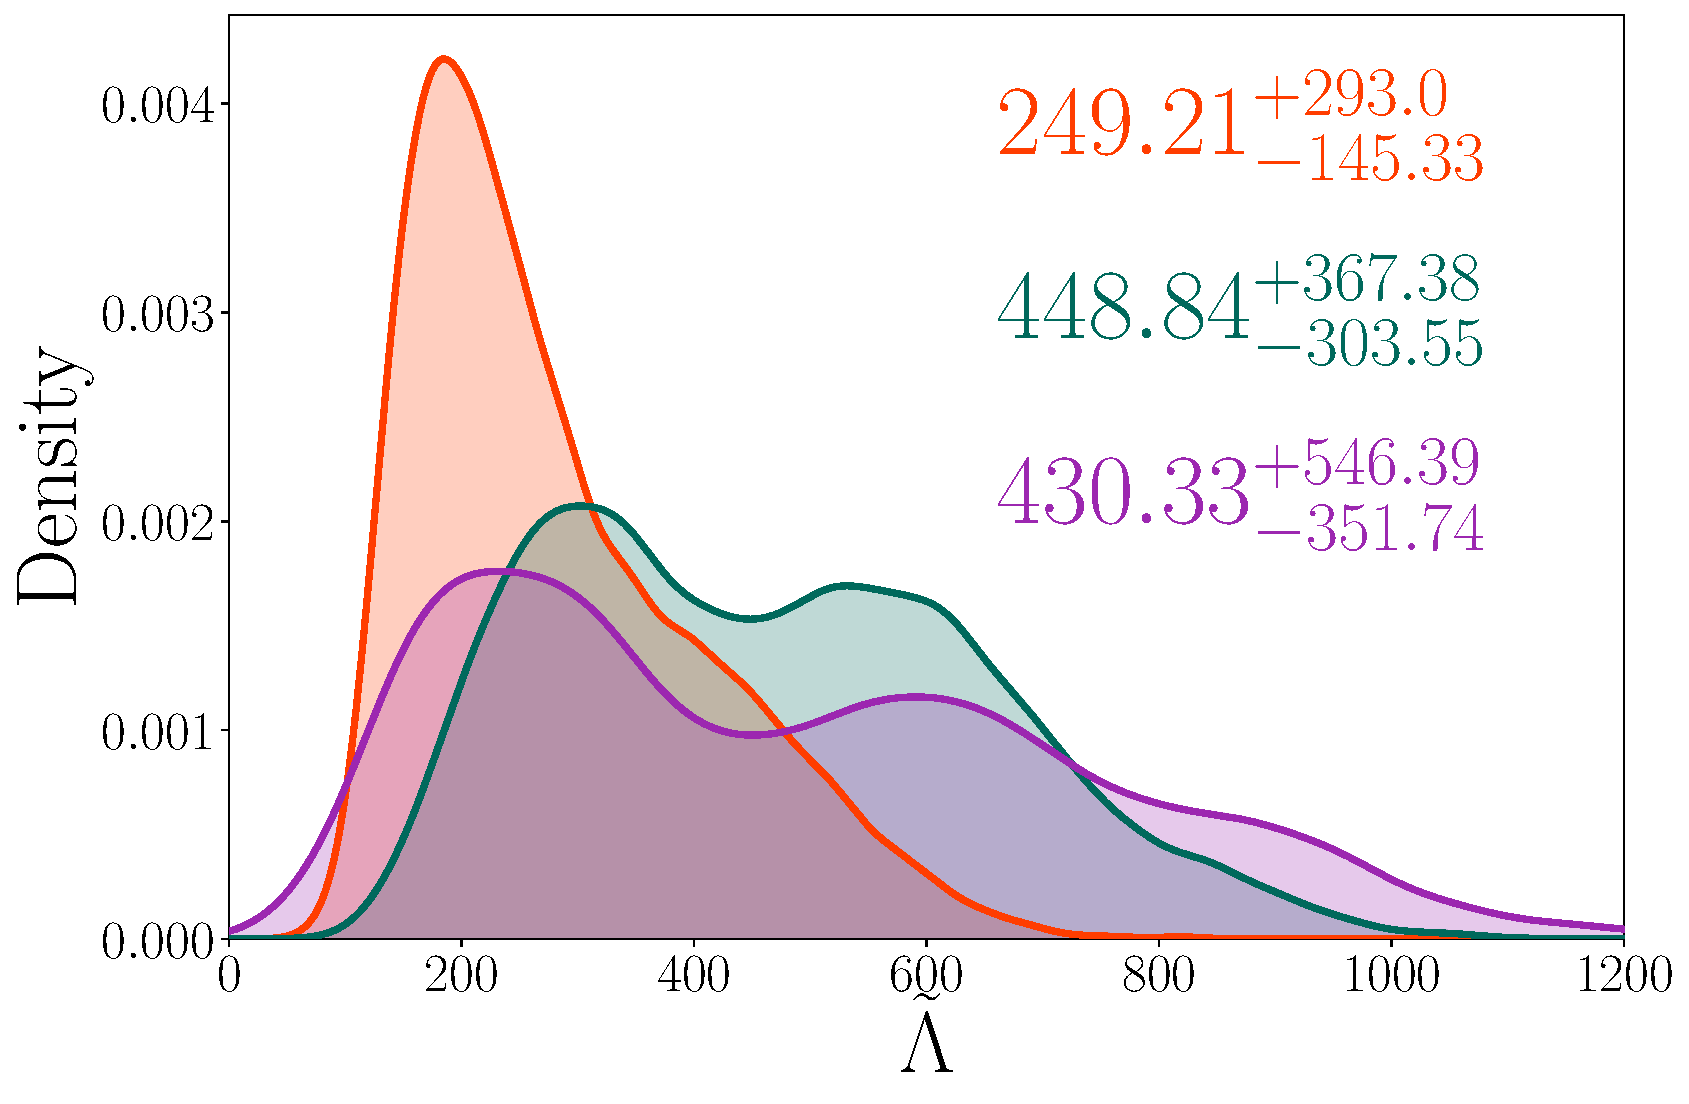
\includegraphics[width=0.95\linewidth]{Figures/GW170817.pdf}
    \end{figure}

    \column{.01\textwidth}
    \rule{.2mm}{.8\textheight}

    \column{0.49\textwidth}
    \centering 
    \textbf{GW190425}
    \vspace{\x}
    \begin{align*}
      ln \ \bayesfactor^{\jaxtwo{\rm{BNS}}}_{\nsbh{\rm{NSBH}}} &= \phantom{-}4.13 \\
      ln \ \bayesfactor^{\jaxtwo{\rm{BNS}}}_{\jaxthree{\rm{agnostic}}} &= -0.30
      % ln \ \bayesfactor^{\nsbh{\rm{NSBH}}}_{\jaxthree{\rm{agnostic}}} &= -4.44 \\
    \end{align*}

    \vspace{\y}

    \begin{figure}
      \centering
      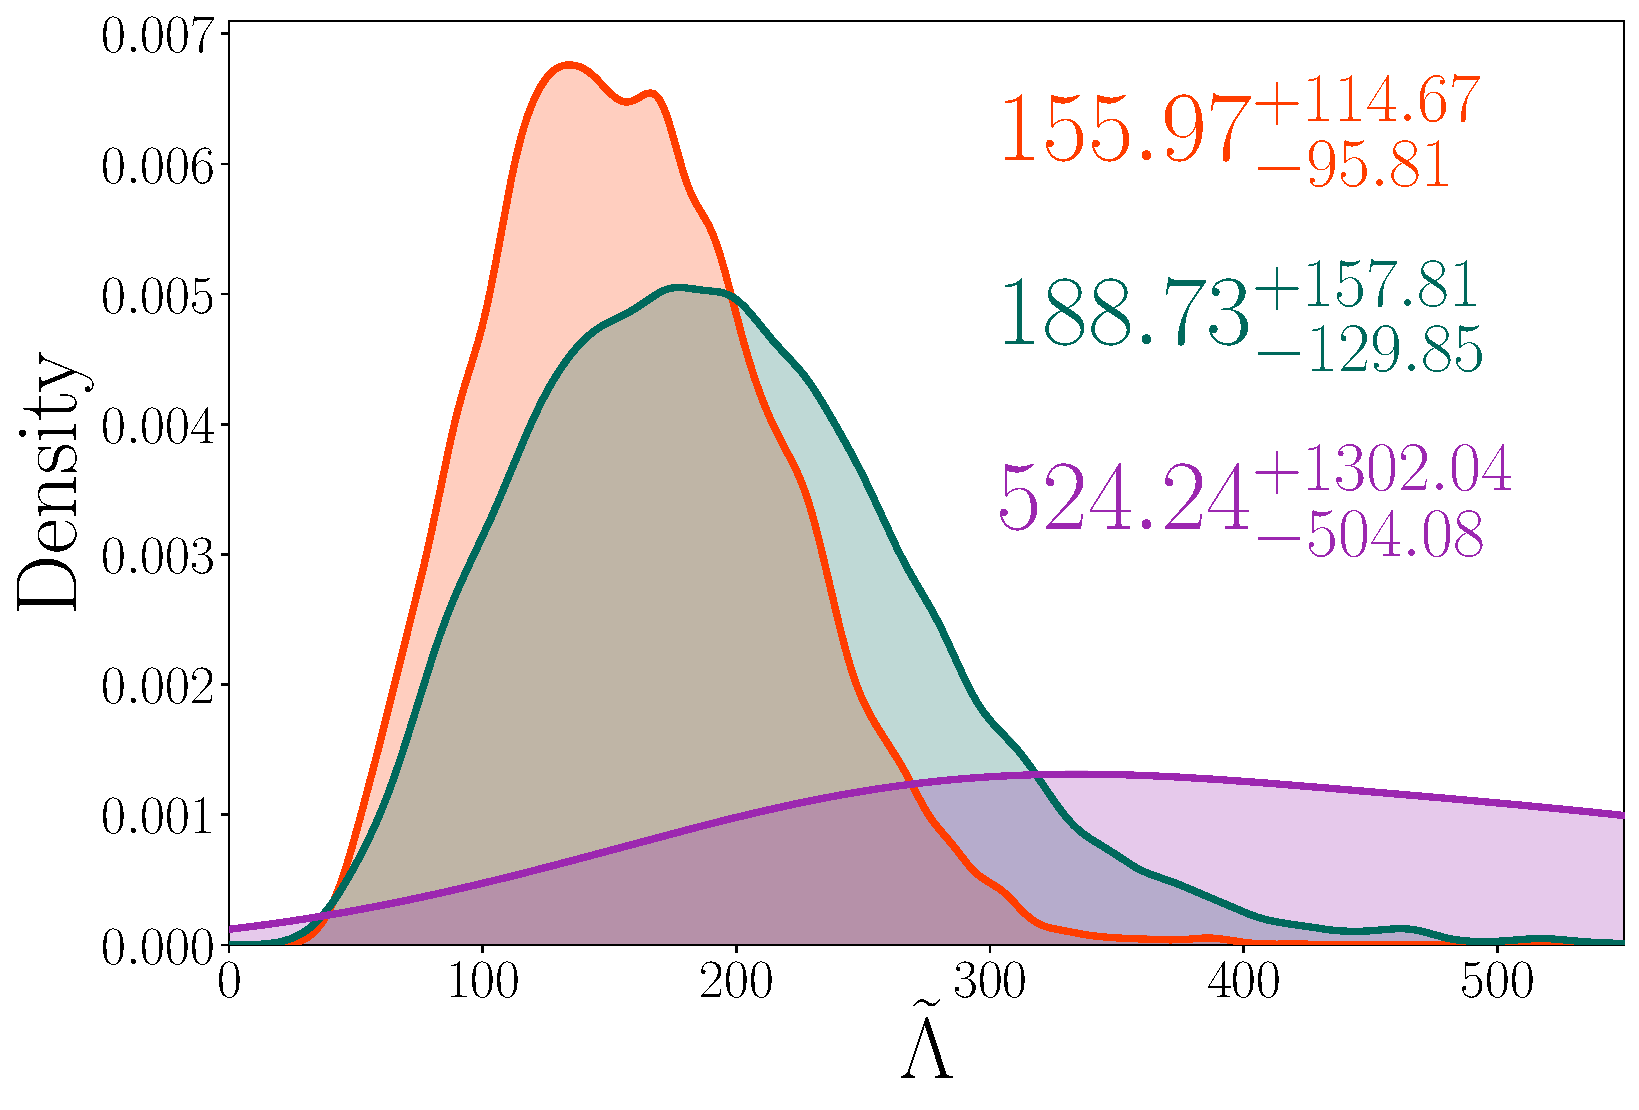
\includegraphics[width=0.95\linewidth]{Figures/GW190425.pdf}
    \end{figure}
  \end{columns}
\end{frame}


\begin{frame}{Source classification: proof of concept}
  \def\x{3mm}
  \def\y{-5mm}

  \begin{columns}[T]
    \column{0.49\textwidth}
    \centering 
    \textbf{GW190425}
    \begin{itemize}
      \item $M_{\rm{max}} > 2 M_\odot$
    \end{itemize}
    \vspace{\x}
    \begin{align*}
      ln \ \bayesfactor^{\jaxtwo{\rm{BNS}}}_{\nsbh{\rm{NSBH}}} &= \phantom{-}4.13 \\
      ln \ \bayesfactor^{\jaxtwo{\rm{BNS}}}_{\jaxthree{\rm{agnostic}}} &= -0.30
    \end{align*}

    \vspace{\y}

    \begin{figure}
      \centering
      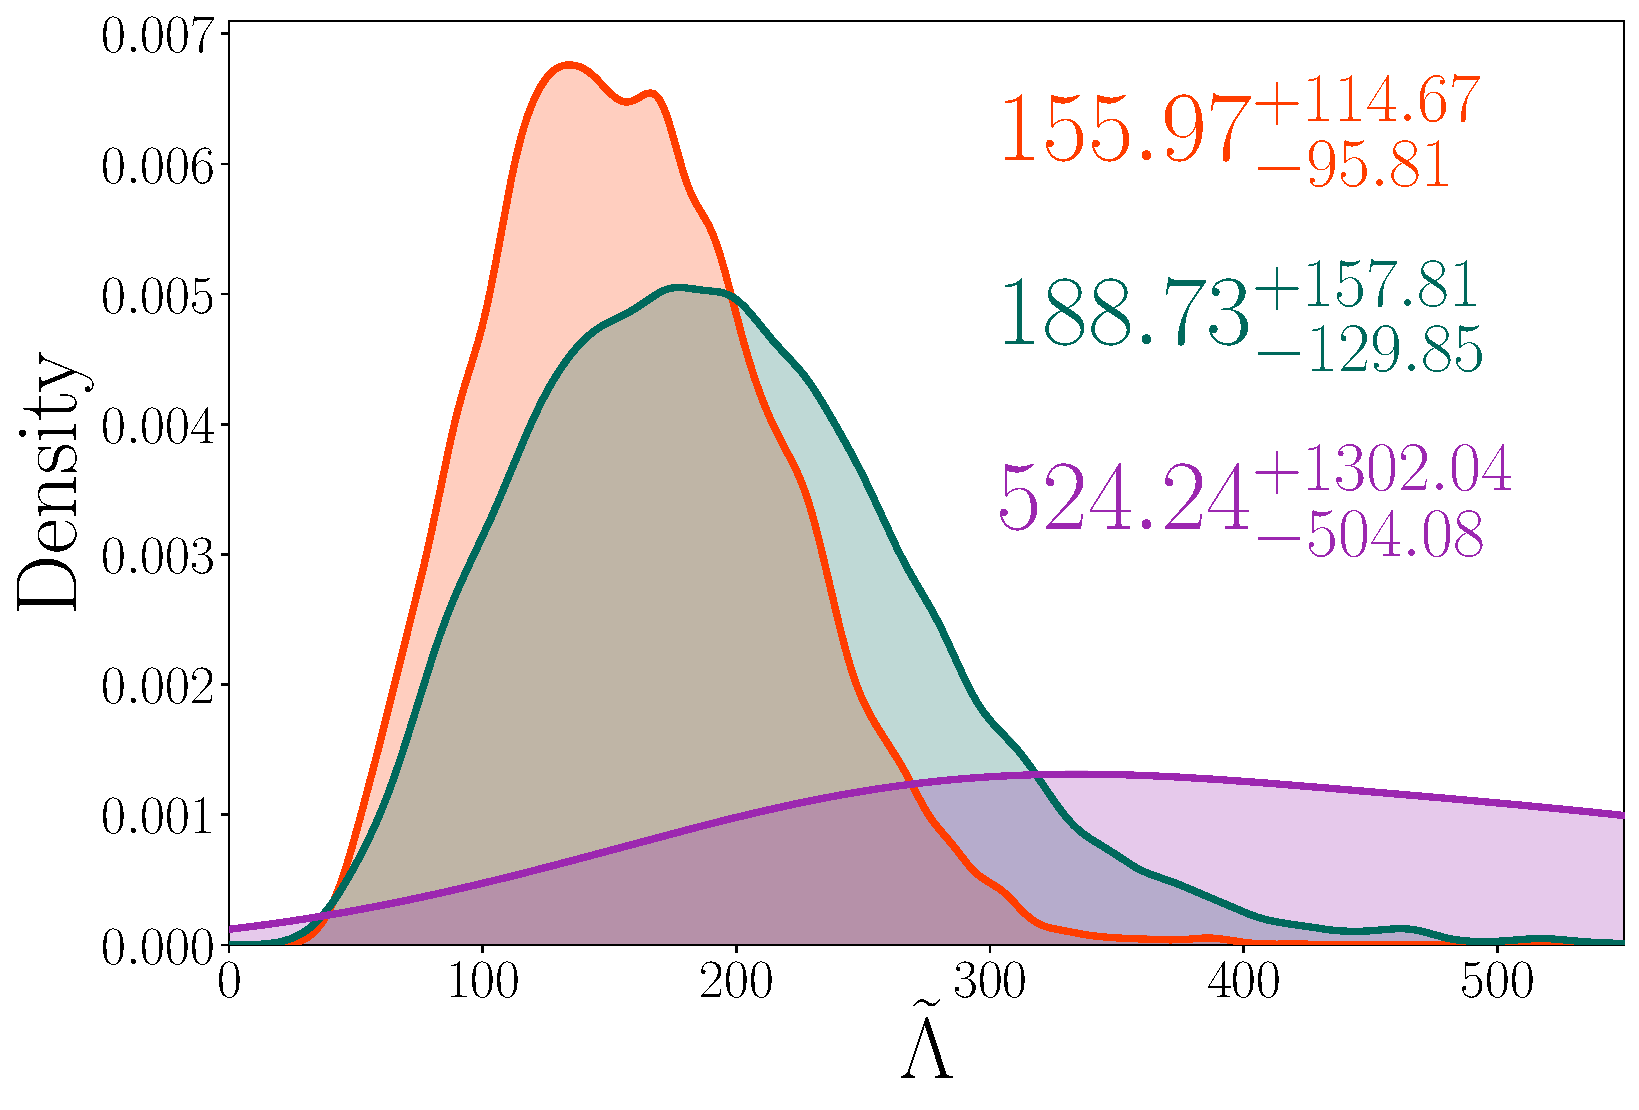
\includegraphics[width=0.95\linewidth]{Figures/GW190425.pdf}
    \end{figure}

    \column{.01\textwidth}
    \rule{.2mm}{.8\textheight}

    \column{0.49\textwidth}
    \centering 
    \textbf{GW190425} 
    \begin{itemize}
      \item[+] mass-radius measurements
      \item[+] GW170817
      \item[+] nuclear theory predictions
    \end{itemize}
    % \vspace{\x}
    \begin{align*}
      ln \ \bayesfactor^{\jaxtwo{\rm{BNS}}}_{\nsbh{\rm{NSBH}}} &= 8.20 \\
      ln \ \bayesfactor^{\jaxtwo{\rm{BNS}}}_{\jaxthree{\rm{agnostic}}} &= 0.28
    \end{align*}

    \vspace{\y}

    \begin{figure}
      \centering
      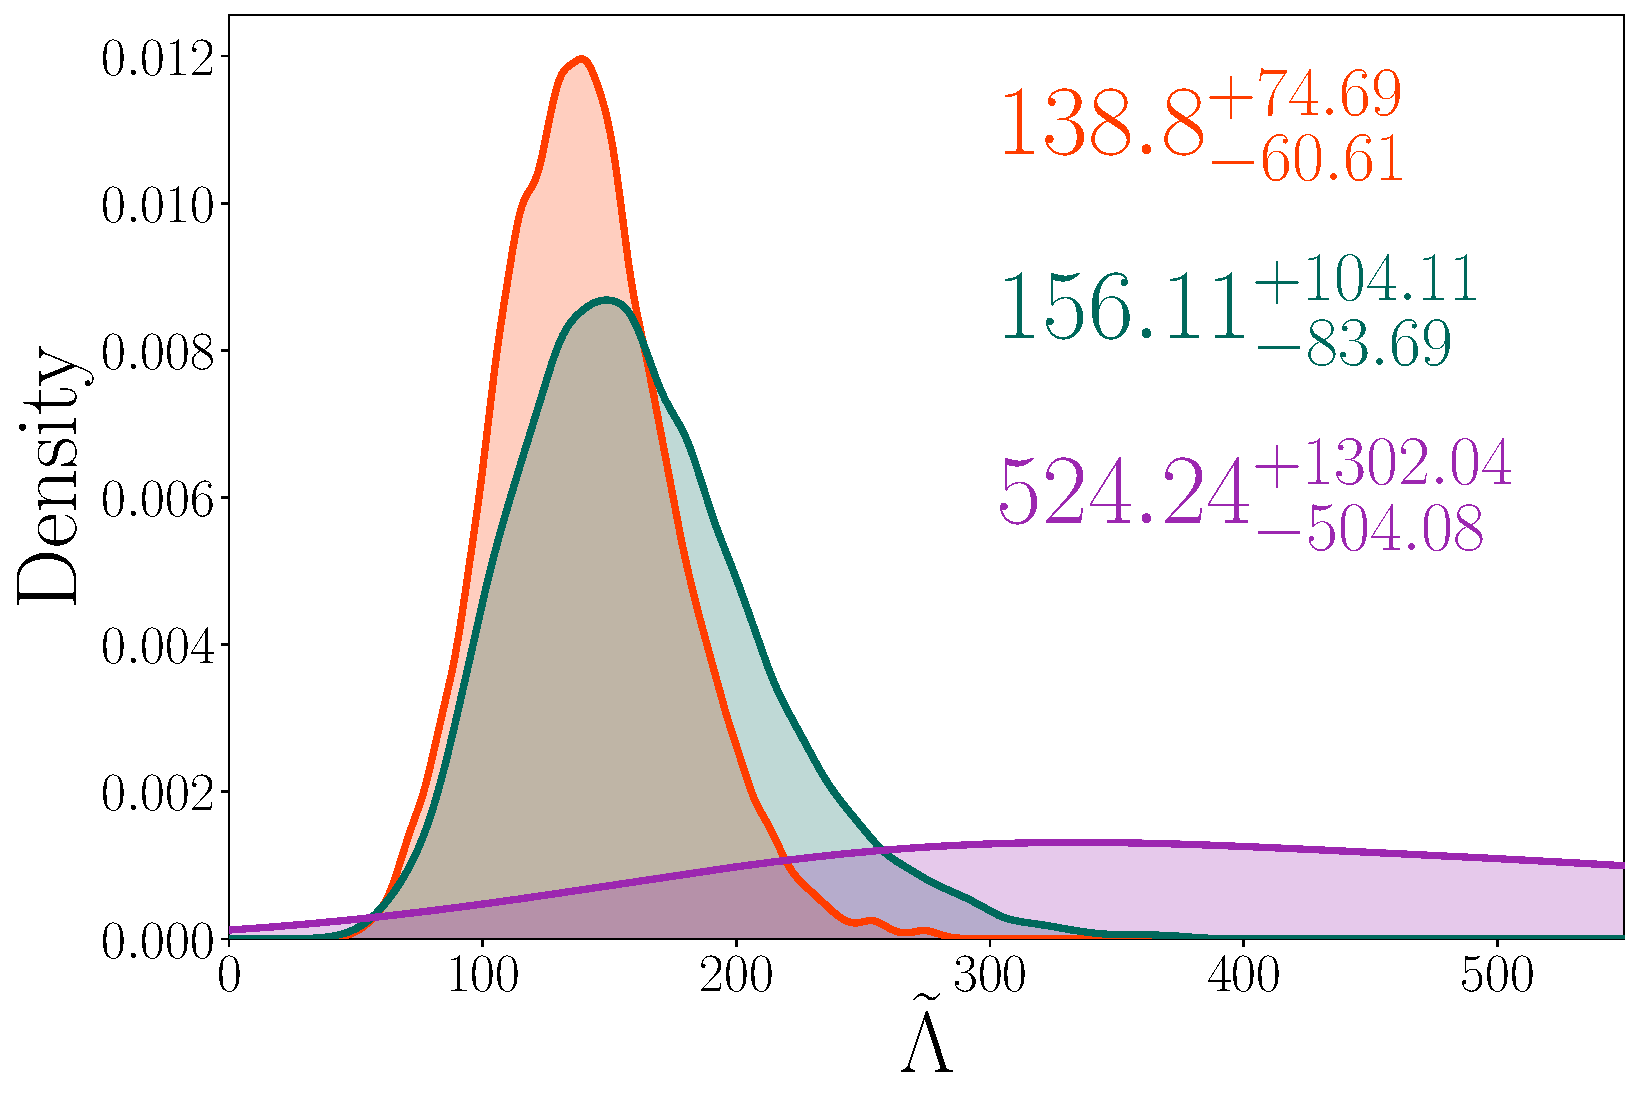
\includegraphics[width=0.95\linewidth]{Figures/GW190425_all.pdf}
    \end{figure}
  \end{columns}
\end{frame}

\begin{frame}{Conclusion}
  \def\x{3mm}

  \centering
  \incfig[0.75\textwidth]{NS_to_EOS_small}

  \begin{itemize}
    \item Neutron star observations and EOS constraints form a data analysis loop

    \vspace{\x}

    \item Constraining EOS: TOV solvers can be accelerated with \textsc{Jax}, avoiding the need for machine learning surrogates

    \vspace{\x}

    \item Applying EOS: Normalizing flows can emulate priors on source parameters informed by EOS knowledge 
    
    \vspace{\x}

    \item Equation of state-informed priors enable source classification: confidence depends on EOS constraints
  \end{itemize}

\end{frame}

\begin{frame}[allowframebreaks]{References}
  \printbibliography
\end{frame}

\appendix 

\begin{frame}{Normalizing flows}
  \def\x{2mm}
  
  \begin{itemize}
    \item Trainable, bijective transformation between \blue{latent} and \red{data} space

    \vspace{\x}

    \item Emulate complicated distributions, trained from samples
  \end{itemize}

  \incfig[\textwidth]{NF}
\end{frame}

\begin{frame}{Projection: 20 BNS in O5}
  \def\x{3mm}

  \begin{itemize}
    \item 20 binary neutron star signals observed with HLV and O5 sensitivity
    \begin{itemize}
      \item Parameter estimation done with \textsc{Jim}~\cite{Wong:2023lgb, Wouters:2024oxj}: $\sim 30$ mins/event
      \item \textbf{\jaxthree{Agnostic}} vs \textbf{\jaxtwo{data-driven}} priors
    \end{itemize}

    \vspace{\x}

    \item Use resulting GW posteriors to constrain the EOS
    \begin{itemize}
      \item $\sim 1$ hour with \textsc{Jester}~\cite{Wouters:2025zju}
    \end{itemize}

    \vspace{\x}

    \item Result: constraints more robust
  \end{itemize}

  \vspace{\x}

  \begin{figure}
    \centering
    \begin{subfigure}[t]{0.475\textwidth}
        \centering
        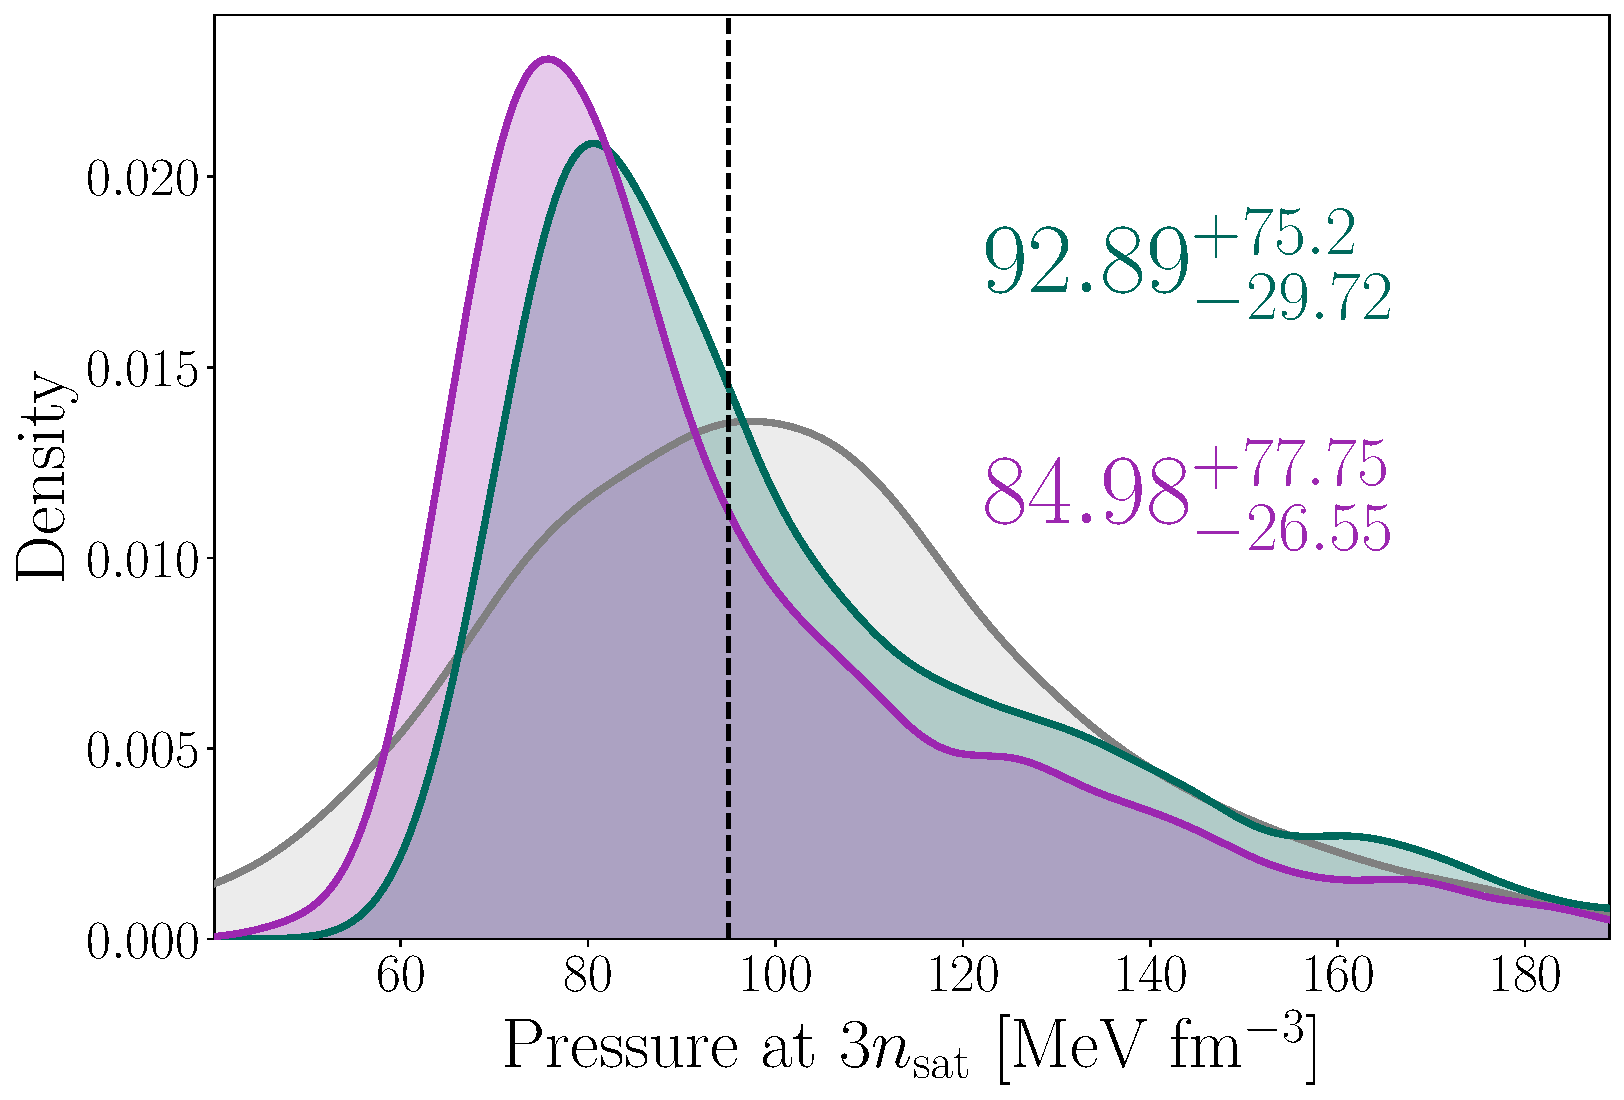
\includegraphics[width=\textwidth]{Figures/p3nsat.pdf}
    \end{subfigure}
    \hfill
    \begin{subfigure}[t]{0.475\textwidth}
        \centering
        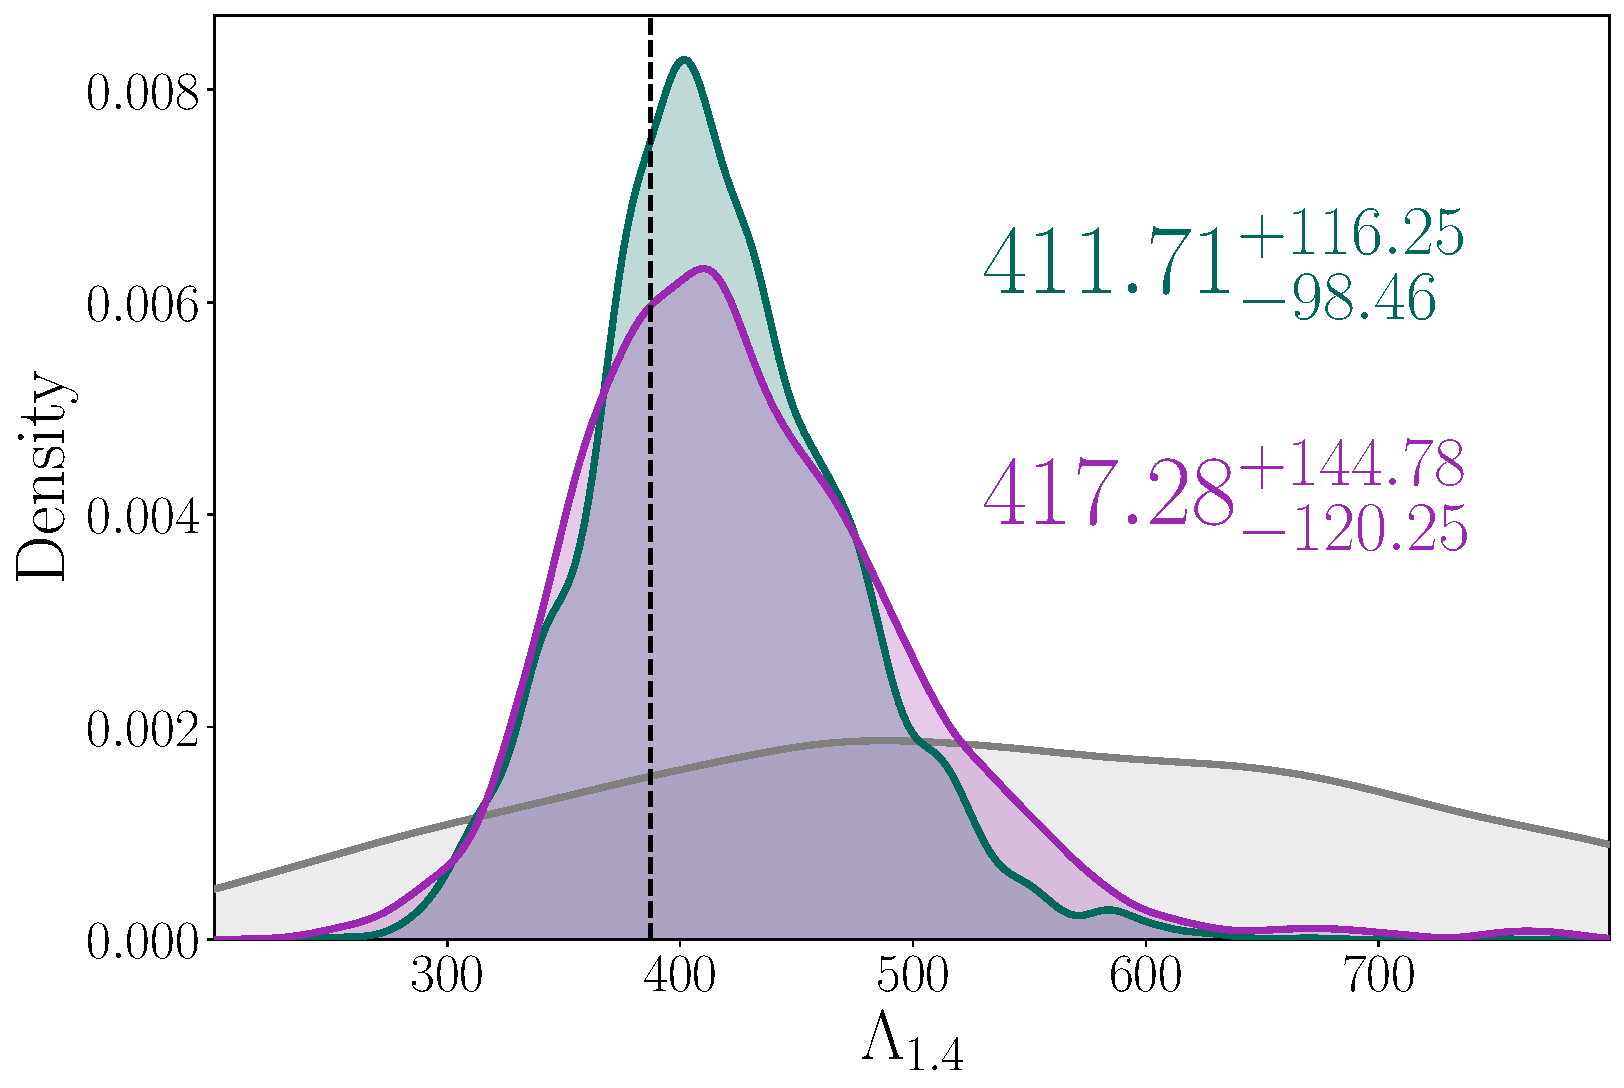
\includegraphics[width=\textwidth]{Figures/l14.pdf}
    \end{subfigure}
  \end{figure}
\end{frame}

\end{document}
